\subsection{Data Collection}

In this section the approach and implementation of data collection for this project is 
examined.

\subsubsection{Requirements for the dataset}

Basic requirements the dataset should fulfill are

\begin{itemize}
    \item \textbf{Includes Spotify song features}

    Spotify provides a set of song features that were generated using their own models.
    The dataset should inlude these features, as they are needed to train the model
    \item \textbf{Includes genre as label}

    The dataset needs to include the genre of the track to use as a label for the classifier
    \item \textbf{Has sufficient sample size per genre}

    In order to train the model well, a sufficient sample size is needed per genre.
    It was not known before collecting the data, how many samples were enough. 
    \item \textbf{Song and Artist name}

    The best way to filter out duplicates is to use the song and artist names.
    Spotify does provide a track id for each song, however, if a song is released twice
    (e.g. as a single and later in an album), these track ids will differ which will lead to a duplicate entry.
\end{itemize}

Additional fields are not going to be used in this analysis, but might still be collected in order to publish the
dataset and enable others to use it for different applications.

\subsubsection{Existing Datasets}

As this paper examines creating a model specifically on Spotify Song Data,
a search on the internet was conducted first, to find a potential pre-made dataset,
pulled from the Spotify \ac{API}, which could be used.
Kaggle \footnote{Kaggle Website: https://www.kaggle.com/} lists an extensive
catalogue of community provided datasets, so the main sources of this search were
Kaggle and Google search for the term "Spotify Song Data".
Kaggle lists a couple of datasets that could be applicable to the research question in
this paper. Some examples of datasets listed are given and explained, why they could not 
be used for this project.

"Spotify music analysis" by user Aeryan \footnote{https://www.kaggle.com/aeryan/spotify-music-analysis}
is a dataset of 2017 rows, which includes musical features like acousticness and tempo,
the song title and artist, but lacks a genre field. Because of the small sample size
and the missing genre field, this dataset could not be used.

There are multiple datasets which include songs that were featured in Spotify's "Top 50" Playlists,
charts, or year in review, recorded at a single point in time or historically.
\footnote{https://www.kaggle.com/nadintamer/top-spotify-tracks-of-2018}
\footnote{https://www.kaggle.com/leonardopena/top50spotify2019}
These could not be used, as the sample size is again too small and the focus is specifically
on the most popular tracks and not a wide variety of music in a genre.

"Dataset of songs in Spotify" \footnote{https://www.kaggle.com/mrmorj/dataset-of-songs-in-spotify}
is the most promising dataset examined, as it has a big sample size and includes genre data.
However, the methodology of how the data was collected is not included and there
could be multiple ways of how genre data for a given song is collected, as is explained later.
Also the genres are limited to very specific directions of Electronic Dance Music and Hip-Hop.

As no optimal dataset for this research paper could be found using our search criteria,
a dataset was specifically created for this paper using the Spotify Web API.

\subsubsection{Ressources and Approach}

Spotify provides extensive documentation for developers on their developer website \footnote {https://developer.spotify.com/}.
This includes development and design guidelines for teams, that want to integrate
Spotify's service into their own apps, documentation on IOS and Android development
a community forum, a developer dashboard and the Web API documentation, which is the main ressource
for data collection from Spotify.

The \ac{API} is based on the \ac{REST} architecture. The different endpoints return JSON metadata
directly from the Spotify Data Catalogue \cite[]{SpotifyWebAPI}. There are also features to query for
user related data using an authorization flow with the users Spotify account, but this is not relevant
in this context. \cite{SpotifyWebAPI} Requests to the \ac{API} are made via HTTPS GET or POST methods.
The \ac{API} can be used by anyone, but authorization via the OAuth protocol is required to access data
from the \ac{API}. 
To explore the \ac{API} and find endpoints to use, Spotify provides a developer console, which can be used to 
send requests and see what kind of responses come back. This is not suitable for saving the data or making multiple
requests programmatically, but is helpful for API exploration. As there is not one single endpoint that delivers all
required fields, multiple queries that build on top of each other have to be made.

The approach began with using the \ac{API} reference to get an overview over the endpoints and their responses.
The specific endpoints that might return interesting data were queried using the Spotify Web Console, to see
a response with live data and which exact fields are returned.
Beyond the Web Console, the tool "Postman" was used to explore the \ac{API}.
It is a platform that can be used to make HTTP requests to an API and store these requests in
a collaborative environment. \cite{PostmanWhatIs} It supports the required authorization workflows
and enabled the research team to explore endpoints together, easily make \ac{API} calls without having to
authenticate by hand, and save the endpoints and required input parameters in a shared workspace.
Once exploration was complete, the complete data collection was implemented in Python 3, mainly using the
libraries http, json and requests. The final result was saved as a CSV file to be used for data exploration
and further processing.

Many API endpoints give the option to specify a country and locale that the results should apply to.
Whenever possible these values were explicitly specified to eliminate the risk of receiving data for multiple different
countries or languages, which would have made the dataset incoherent.
For country, we used the country tag "US" which means that the API replies only with datapoints that are applicable
to users in the United States of America.
For locale we used en\_US in order to receive the data in the english language.
These two values differ in that country changes the actual entries from the database that are selected for the response
and sent to the users. Locale defines in which language these selected entries are returned in.

\subsubsection{Authorization}

Using the Spotify documentation for authorization workflows \cite{SpotifyAuth}, authorization was first tested
using Postman and then implemented in Python.
The workflow is explained using the Python code.
Using a Spotify account to log in, the developer dashboard can be accessed. Here an application was registered with
Spotify for the research project. Spotify tracks \ac{API} usage per application and can recognize if the API is
being abused or too many requests are sent, which will result in rate limitation or blocking.
On the API Dashboard, a "Client ID" and "Client Secret" can be retrieved. These credentials are used to start
the authorization flow, as described by Spotify in Figure \ref{fig:Spotify Authorization Flow}.

\begin{figure}[H]
    \caption{Spotify Authorization Flow}
	\label{fig:Spotify Authorization Flow}
    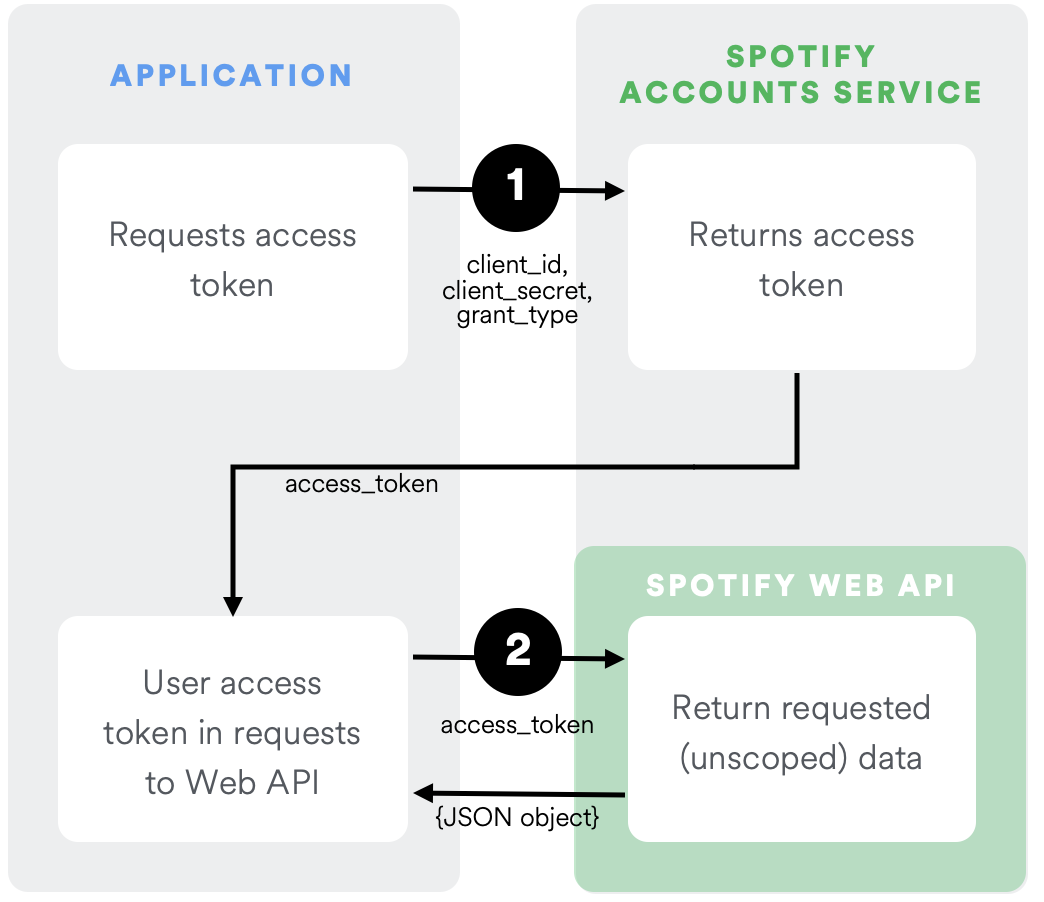
\includegraphics[width=0.6\textwidth]{SpotifyAuthFlow}
    \\
    Source: \cite{SpotifyAuth}
\end{figure}

Step one is a post request to the Spotify Account Service with the client id and client secret from the application dashboard, which returns an
access token, that is valid for one hour. This token can be used to access any endpoint of the actual \ac{API} that
does not require user specific data. When the token expires, a new one has to be requested before querying the \ac{API} again.
Figure \ref{fig:Access Token Request} shows the full request and response to acquire the token.

\begin{figure}[H]
    \caption{Access Token Request}
	\label{fig:Access Token Request}
\begin{apiRoute}{post}{https://accounts.spotify.com/api/token}{request access token}
    \begin{routeRequest}{application/x-www-form-urlencoded}
        \begin{routeRequestBody}
{
    "grant_type": "client_credentials",
    "client_id": client id from application dashboard,
    "client_secret": client secret from dashboard
}
        \end{routeRequestBody}
    \end{routeRequest}
    \begin{routeResponse}{application/json}
        \begin{routeResponseItem}{200}{ok}
            \begin{routeResponseItemBody}
{
    "access_token": "BQDgQCSx-tIMDo9LfVeZxm6YMl2p_WbEU3Q9ENsVl7e--6d_vockTsfzMVUhPWiHSSnFUuHvm_9POA1kYEw",
    "token_type": "Bearer",
    "expires_in": 3600
}
            \end{routeResponseItemBody}
        \end{routeResponseItem}
    \end{routeResponse}
\end{apiRoute}
\end{figure}


\subsubsection{Getting Features}

In order to predict the genre of a track based on audio features, these features have to be requested
for every track. Spotify provides an endpoint to get audio features for a single track or up to 99 tracks at
a time. The latter is used in the Python implementation as it reduces the number of requests to be made.
The typical request/response pattern for the audio-feature request endpoint is shown in
figure \ref{fig:Audio Feature Request}.

\begin{figure}[H]
    \caption{Audio Feature Request}
	\label{fig:Audio Feature Request}
\begin{apiRoute}{get}{https://api.spotify.com/v1/audio-features?ids=\{ids\}}{request audio features for id}
    \methodJson
    \begin{routeParameter}
        \routeParamItem{ids}{comma seperated list of up to 99 song ids}
    \end{routeParameter}
    \begin{routeResponse}{application/json}
        \begin{routeResponseItem}{200}{ok}
            \begin{routeResponseItemBody}
{
    "audio_features": [
        {
            "danceability": 0.677,
            "energy": 0.638,
            "key": 8,
            "loudness": -8.631,
            "mode": 1,
            "speechiness": 0.333,
            "acousticness": 0.589,
            "instrumentalness": 0,
            "liveness": 0.193,
            "valence": 0.435,
            "tempo": 82.810,
            "type": "audio_features",
            "id": "2e3Ea0o24lReQFR4FA7yXH",
            "uri": "spotify:track:2e3Ea0o24lReQFR4FA7yXH",
            "track_href": "https://api.spotify.com/v1/tracks/2e3Ea0o24lReQFR4FA7yXH",
            "analysis_url": "https://api.spotify.com/v1/audio-analysis/2e3Ea0o24lReQFR4FA7yXH",
            "duration_ms": 211497,
            "time_signature": 4
        },
        ...
    ]
}
            \end{routeResponseItemBody}
        \end{routeResponseItem}
    \end{routeResponse}
\end{apiRoute}
\end{figure}

With the exception of type, id, uri, track\_href and analysis\_url, all of the fields included in this response
can be used as features in the dataset. However, this api call expects a track id, which we need to get using
other api calls first. This could be a search endpoint, getting all tracks in a playlist, etc.
Also, it does not give the track or artist names and doesn't include a genre.

\subsubsection{Getting Track IDs and Labels}

There is no simple endpoint that takes one or more track ids and returns  a "genre" field
in its response. The exploration of the API using the reference, web console and Postman only revealed
two ways of getting the genre of a track. 

The first way is using the artist of a track. Given a track id, the artists of the track and their corresponding
ids can be requested by using the "/tracks/{id}" endpoint. Then, using the artist id, the genres that an
artist is known for are returned, as can be seen in figure \ref{fig:Artist Request}.

\begin{figure}[H]
    \caption{Artist Request}
	\label{fig:Artist Request}
\begin{apiRoute}{get}{https://api.spotify.com/v1/artists/\{id\}}{request information about an artist by their id}
    \begin{routeParameter}
        \routeParamItem{id}{id of the artist}
    \end{routeParameter}
    \begin{routeResponse}{application/json}
        \begin{routeResponseItem}{200}{ok}
            \begin{routeResponseItemBody}
{
    "external_urls": {
        "spotify": "https://open.spotify.com/artist/6l3HvQ5sa6mXTsMTB19rO5"
    },
    "followers": {
        "href": null,
        "total": 15554811
    },
    "genres": [
        "conscious hip hop",
        "hip hop",
        "north carolina hip hop",
        "rap"
    ],
    "href": "https://api.spotify.com/v1/artists/6l3HvQ5sa6mXTsMTB19rO5",
    "id": "6l3HvQ5sa6mXTsMTB19rO5",
    "images": [
        ...
    ],
    "name": "J. Cole",
    "popularity": 89,
    "type": "artist",
    "uri": "spotify:artist:6l3HvQ5sa6mXTsMTB19rO5"
    }
            \end{routeResponseItemBody}
        \end{routeResponseItem}
    \end{routeResponse}
\end{apiRoute}
\end{figure}

This examplary API response shows a problem with this approach. One artist can be sorted
into multiple genres.
A given track might be associated with either of the artists genres, but the data does
not show, which one exactly.
Additionally a track might have multiple artists which further complicates this.
Given these circumstances, this approach is problematic.

The second way is Spotifys "categories" feature. The apps search tab provides a number of
categories that a user can browse through to find new music in their preferred genre or style.
In figure \ref{fig:Categories and Playlists in Spotify App}a an overview over some of the categories
that are available in the Spotify App is shown. There are categories of multiple types, e.g.
specific activities, like Cooking or Gaming, or places, like "At Home" or "In the Car".
But there are also categories for nearly all major genres. In the app screenshot
there is for example Classical, Jazz or Soul.
These categories can be used to get tracks that belong in each specific category. When a user taps on
one of the categories, playlists that contain tracks of the respective category are shown to the user,
like shown in figure \ref{fig:Categories and Playlists in Spotify App}b.

\begin{figure}[H]
    \centering
    \subfloat[\centering Category Overview]{{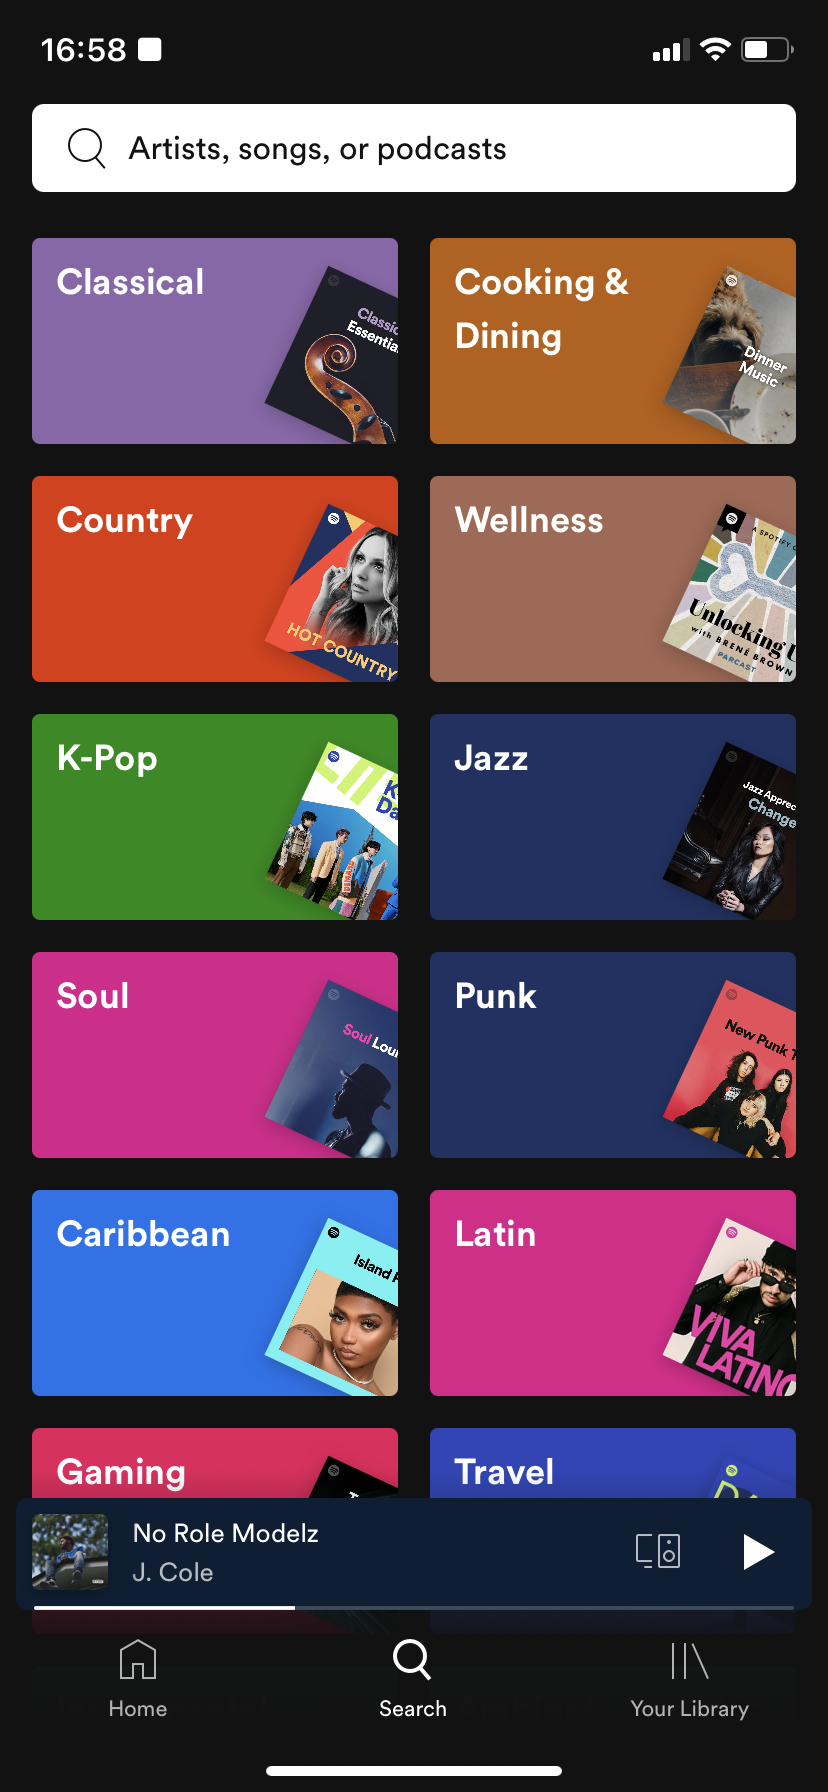
\includegraphics[width=4cm]{SpotifyCategoryOverview} }}%
    \qquad
    \subfloat[\centering Playlists in category]{{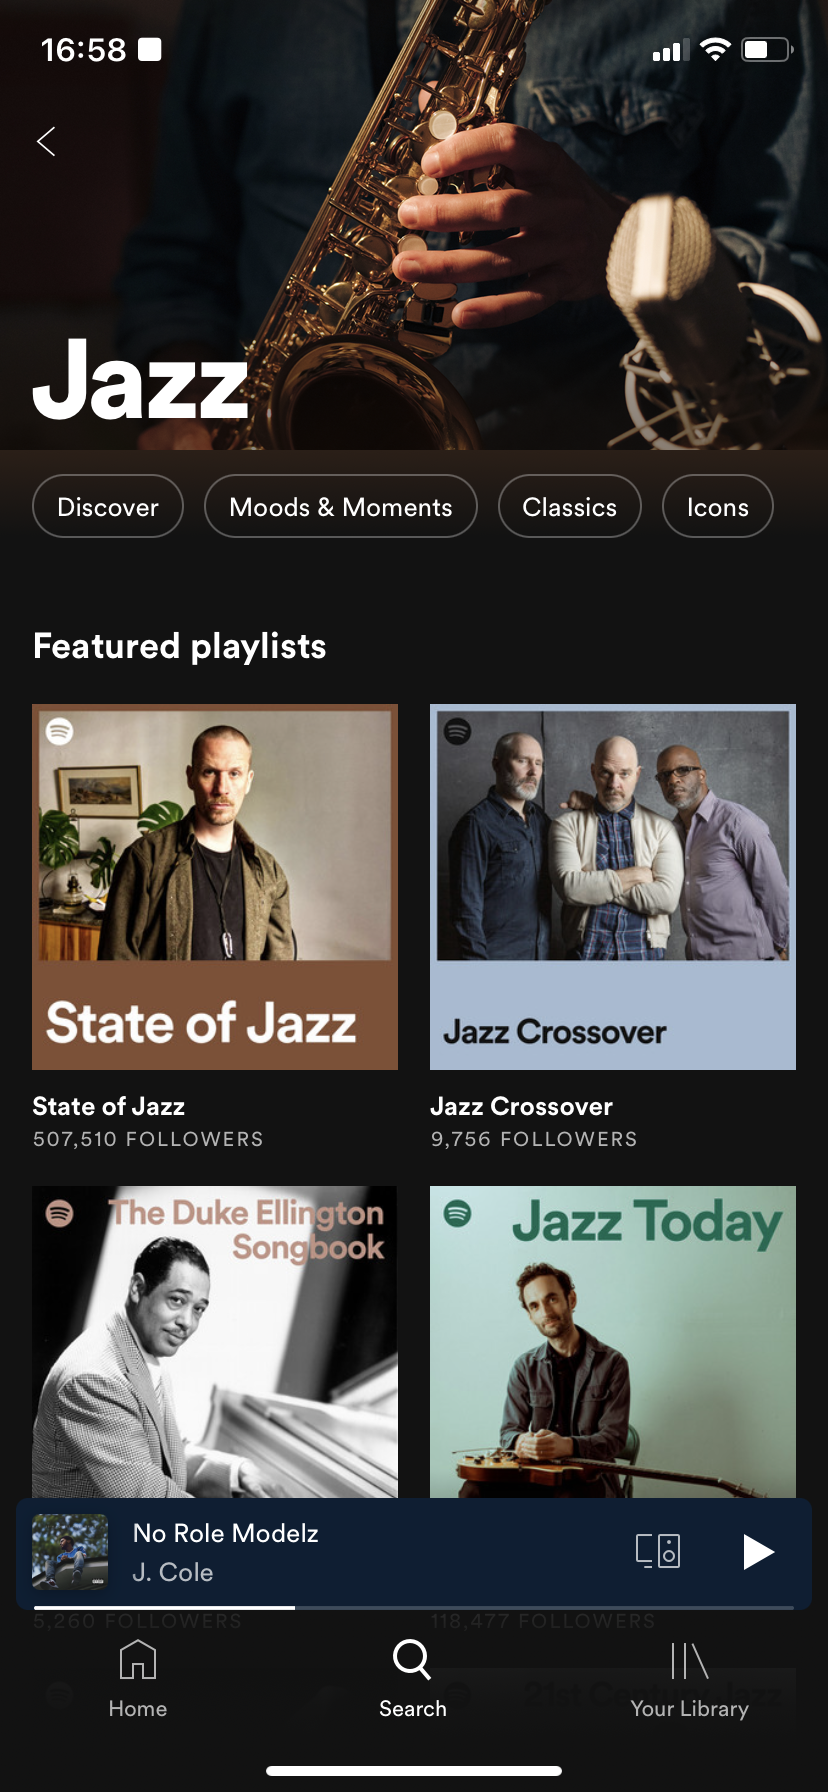
\includegraphics[width=4cm]{SpotifyPlaylistOverview} }}%
    \caption{Categories and Playlists in Spotify App}%
    \label{fig:Categories and Playlists in Spotify App}%
\end{figure}

The API mirrors the apps behaviour and provides an endpoint to get a list of categories and their ids,
one to get all playlists and playlist\_ids in a category, and one to get all tracks and track\_ids in
a playlist. This chain of API calls is used to request every track in every playlist in a certain category.


\subsubsection{Python Implementation}

This section describes, how the previously explained API-Calls are used to request data from the API
and save the complete dataset as a CSV file. The script was implemented in a way that lets anyone with a registered Spotify
developer application run it to gather their own data.
It supports filtering for certain genres to speed up the process and exporting the current data after each step
to be able to pause the data collection and check the current results or continue later.
The details of these functions are explained in this section using code snippets.

The Python requests library is used to execute the requests, as it supports the features needed to send the GET and POST
requests we need without having to write complicated code.
The dotenv library is used to read the client id and secret from a seperate .env file, rather than writing it into the code.
This prevents these sensitive credentials from being committed into version control,
which is hosted in a public GitHub repository and would therefore make the credentials public.
The "json" library is used for transforming Python dictionaries into json data, "math" for access to rounding functions,
"os" for managing system paths and access to files, "http" to define retry and timeout behaviour of the API-Calls and "csv"
to finally transform the json data into a CSV file.

First, the credentials are read using "load\_dotenv". Then a method is defined which takes the client id and secret as input,
executes a POST request to the accounts API, as shown in \ref{fig:Access Token Request} and return the access token from the
"access\_token" field in the response. 

\begin{lstlisting}[language=Python]
    #Get environment variables from ".env" file and read credentials
    load_dotenv('.env')
    client_id = os.environ.get('CLIENT_ID')
    client_secret = os.environ.get('CLIENT_SECRET')
    
    # Authenticate and get an API Token from Spotify using a Client ID and secret
    def getAuthTokenFromCredentials(id, secret):
    
        url = "https://accounts.spotify.com/api/token"
    
        payload = f'grant_type=client_credentials&client_id={id}&client_secret={secret}'
        headers = {
        'Content-Type': 'application/x-www-form-urlencoded',
        }
    
        response = requests.request("POST", url, headers=headers, data=payload)
    
        return response.json()["access_token"]
    
    auth_token = getAuthTokenFromCredentials(client_id, client_secret)
\end{lstlisting} 

Next the http library is configured to use a ten second timeout and attempt five retries. If a request to the API is made
and no response is given from Spotify's servers after ten seconds, the request will be sent again. If there is still no
answer from the server after five attempts, an Exception is thrown and the script ends.
Timeouts are crucial as short disconnections from the Internet could result in the whole data collection step failing.
The http setup code is found in appendix \ref{appendix:http setup}.

The next part of the script implements the filter mechanism

\begin{lstlisting}[language=Python]
    category_filter = None

    # comment this out if you don't want to set a filter
    category_filter = ["hiphop", "pop", "country", "rock", "latin", "rnb", "mood", "indie_alt",
                        "regional_mexican", "edm_dance", "inspirational", "chill", "party", "roots",
                        "kpop", "instrumental", "ambient", "alternative", "classical", "jazz", "soul",
                        "punk", "blues", "arab", "afro", "metal", "caribbean", "funk"]
    
    # tells data collection functions to not use filter if it's not set
    if category_filter is not None:
        use_filter = True
    else:
        use_filter = False
\end{lstlisting} 

The option to filter the categories that are to be taken into account when collecting the data is given.
Possible values are all valid category ids, which can be requested using the API call shown in figure \ref{fig:Categories Request}

\begin{figure}[H]
    \caption{Categories Request}
	\label{fig:Categories Request}
\begin{apiRoute}{get}{https://api.spotify.com/v1/categories?country=\{country\}\&locale=\{locale\}\&limit=\{limit\}\&offset=\{offset\}}{Get a list of categories used on Spotifys browse tab}
    \begin{routeParameter}
        \routeParamItem{id}{id of the artist}
        \routeParamItem{country}{only display categories available in a specific country}
        \routeParamItem{locale}{the language in which the categories should be returned}
        \routeParamItem{limit}{the maximum number of items to be returned}
        \routeParamItem{offset}{index of the first item to return}
    \end{routeParameter}
    \begin{routeResponse}{application/json}
        \begin{routeResponseItem}{200}{ok}
            \begin{routeResponseItemBody}
{
    "categories": {
        "href": "...",
        "items": [
            {
                "href": "...",
                "icons": [
                    {
                        "height": 274,
                        "url": "...",
                        "width": 274
                    }
                ],
                "id": "hiphop",
                "name": "Hip-Hop"
            },
            {
                "href": "...",
                "icons": ...
                "id": "pop",
                "name": "Pop"
            },
            ...
        ],
        "limit": 10,
        "next": "...",
        "offset": 0,
        "previous": "...",
        "total": 58
    }
}
            \end{routeResponseItemBody}
        \end{routeResponseItem}
    \end{routeResponse}
\end{apiRoute}
\end{figure}

The response shows an id field for each item in the items array. These ids can be used in the filter list.
If the category\_filter variable is undefined, no filter is set.

Next, the option to import existing data from a file is given.
If a user already has the json data containing all playlists for all categories they want to use,
they can load the json file here and skip executing the collection of categories and playlists and continue right
at the collection of tracks for each playlist.

\begin{lstlisting}[language=Python]
    data = {}

    #To load data_object from file instead of rerunning the scripts, uncomment this:

    file = open(os.path.join("data_collection", "json", "tracks_full.json"))
    data = json.load(file)
\end{lstlisting} 

Next, the four main steps of data collection will be defined and executed:

\begin{enumerate}
    \item Getting categories
    \item Getting playlists
    \item Getting tracks
    \item Getting audio features
\end{enumerate}

Each step is defined as a function with some input parameters and the resulting json data as output, which can then
be used as input for the next step.

The function definition for getting the categories looks like this:

\begin{lstlisting}[language=Python]
    def getAllCategories(
        requests_session, # takes the requests session, which was set up in the beginning
        auth_token, # this is the token which was retrieved in the authorization step
        use_category_filter=False, # set to True if the category_filter should be used
        category_filter=None,  # this takes the list which is used as a category filter
        write_to_file=False, # set to True if the result of this step should be written into a json file
        path_to_file=''): # give the file path at which the json file should be stored

        ...
\end{lstlisting}

The function first makes a simple API call with limit=1 to get the total amount of categories available.
This is necessary, because the API returns a maximum number of 50 entries per request, so if the total number of
items exceeds 50, multiple calls have to be made.

\begin{lstlisting}[language=Python]
    # Establishing the requests session
    http = requests_session

    # First API call used to get the total amount of categories
    headers = { 'Authorization': f'Bearer {auth_token}' }
    url = "https://api.spotify.com/v1/browse/categories?country=US&locale=en_US&limit=1"
    
    try:
        response = http.request("GET", url, headers=headers, data={})
        if response.status_code != requests.codes.ok:
            raise Exception
    except Exception as e:
        raise SystemExit(e)
\end{lstlisting}

The requests\_session is saved in the http variable. Then the auth\_token is wrapped in an Authorization header
conforming to the OAuth Bearer Token standard, which is used by the API.
The url is given with the right country and locale settings and the request is sent inside of a try block.
If the response doesn't contain an HTTP status code 200, an Exception is raised and the program is stopped,
as there is possibly an error in the request or response which could mean corrupted data.

Next, the total amount of categories is extracted from the response and the number of pages is calculated.

\begin{lstlisting}[language=Python]
    categoryAmount = response.json()["categories"]["total"]

    # API only returns 50 items at a time. Offset can be used to gradually get all items
    # Calculate number of pages with 50 items
    pages = int(math.ceil(categoryAmount/50))
    data = {"categories": []}
\end{lstlisting}

By dividing the category amount by 50 and rounding up to the next integer, the number of API calls necessary to get 
all entries is calculated. We call this pages, like pages in a book. Page one contains items 0 to 49 and is retrieved by
using offset 0 and limit 50. Page two contains items 50 to 99 and is retrieved by using offset 50 and limit 50.
This is done as many times as required. the last page will not necessarily contain 50 items but less, as those are left over.

A for loop is used to execute the request for every page as shown before. The offset is increased by 50 with each run.
Each category's id and name are read from the response and appended to the data object:

\begin{lstlisting}[language=Python]
    for x in range(pages):
        url = f"https://api.spotify.com/v1/browse/categories?country=US&locale=en_US&limit=50&offset={x * 50}"
        
        try:
            response = http.request("GET", url, headers=headers, data={})
            if response.status_code != requests.codes.ok:
                raise Exception
        except Exception as e:
            raise SystemExit(e)
        
        # categories are stored in the data dictionary
        for el in response.json()["categories"]["items"]:
            if (use_category_filter == True and el["id"] in category_filter) or use_category_filter == False:
                data["categories"].append({
                    "id": el["id"], 
                    "name": el["name"]
                })
\end{lstlisting}

Outside of the for loop, the resulting data is written to a file if write\_to\_file was set to True and the 
data object is returned:


\begin{lstlisting}[language=Python]
    if write_to_file == True:
        with open(path_to_file, 'w') as outfile:
            json.dump(data, outfile, indent=2)

    return data
\end{lstlisting}

The data collected after this step looks like this:

\begin{lstlisting}[language=Python]
{
    "categories": [
        {
            "id": "hiphop",
            "name": "Hip-Hop"
        },
        {
            "id": "pop",
            "name": "Pop"
        },
        ...
    ]
}
\end{lstlisting}


This concludes the function getAllCategories.
The data retrieved from this step is used for the next step, getting the playlists.
The function definition here is slightly different:

\begin{lstlisting}[language=Python]
    def getPlaylistsForCategories(
        requests_session,
        auth_token,
        data_object,
        write_to_file=False,
        path_to_file=''):
\end{lstlisting}

Instead of the filtering options, which only apply to the categories, this function takes the data\_object from the
previous step. This could be passed in directly from the previous function or read from a file.
The function implements a nested for loop. The outer loop iterates over all categories in the data object.
The inner loop uses an endpoint to get each category's playlists. The API request/response is shown in figure \ref{fig: Get Category's Playlists Request and Response}.

\begin{figure}[H]
    \caption{Get Category's Playlists Request and Response}
	\label{fig:Get Category's Playlists Request and Response}
\begin{apiRoute}{get}{https://api.spotify.com/v1/categories/\{category\_id\}/playlists?country=\{country\}\&limit=\{limit\}\&offset=\{offset\}}{Get Category's Playlists}
    \begin{routeParameter}
        \routeParamItem{category\_id}{category id}
        \routeParamItem{country}{only display categories available in a specific country}
        \routeParamItem{limit}{the maximum number of items to be returned}
        \routeParamItem{offset}{index of the first item to return}
    \end{routeParameter}
    \begin{routeResponse}{application/json}
        \begin{routeResponseItem}{200}{ok}
            \begin{routeResponseItemBody}
{
    "playlists": {
        "href": "...",
        "items": [
            {
                "collaborative": false,
                "description": "New music from YoungBoy Never Broke Again, DaBaby and 2 Chainz. ",
                "external_urls": ...
                "href": "...",
                "id": "37i9dQZF1DX0XUsuxWHRQd",
                "images": ...
                "name": "RapCaviar",
                "owner": ...
                "primary_color": null,
                "public": null,
                "snapshot_id": "...",
                "tracks": {
                    "href": "https://api.spotify.com/v1/playlists/37i9dQZF1DX0XUsuxWHRQd/tracks",
                    "total": 50
                },
                "type": "playlist",
                "uri": "spotify:playlist:37i9dQZF1DX0XUsuxWHRQd"
            },
            ...
        ],
        "limit": 50,
        "next": "...",
        "offset": 0,
        "previous": null,
        "total": 50
    }
}
            \end{routeResponseItemBody}
        \end{routeResponseItem}
    \end{routeResponse}
\end{apiRoute}
\end{figure}

As there is an upper limit of 50 playlists per request, the same paging method is used as in the category function.
It is checked, if each items "type" field contains the value "playlist", to filter out any items that don't fit the schema.
Then each playlists name and id is stored in the data object, which is returned from the function.
The json data after this step looks like this:

\begin{lstlisting}[language=Python]
{
    "categories": [
        {
        "id": "hiphop",
        "name": "Hip-Hop",
        "playlists": [
            {
            "id": "37i9dQZF1DX0XUsuxWHRQd",
            "name": "RapCaviar"
            },
            {
            "id": "37i9dQZF1DX6GwdWRQMQpq",
            "name": "Feelin' Myself"
            },
            ...
        },
        ...
    }
}
\end{lstlisting}

The third step gets all tracks in each playlist. The function definition is the same as before, as this function also
takes data from the previous step. This time, there are three nested for loops. One for looping through the categories,
then another one for looping through the playlists. In this one there is again calculated how many pages of 50 tracks
need to be requested and the third loop requests the pages and appends the tracks to the playlist data.
The request parameters for this request differ from the other steps. Instead of country, there is a market parameter,
which essentially does the same thing. There is also a fields parameter, which takes a string that can be used to
define which fields the API should return. This is done to save bandwith, as the response of this endpoint is very large and most
of the datapoints might not be needed by the client.
In this case, the value "items(track(name, id, album(name, id), artists)), total" is used to return only items of type track,
their id and name, their albums name and id, and their artist information. Also the total amount of tracks in the playlist is returned.
There is also an "additional\_types" parameter, which can be used to specify if only music tracks, or also podcast episodes should be returned.
In this case, only tracks are returned as podcasts are irrelevant to our analysis.
An examplary API request/response using the described "fields" and "additional\_types" parameters is shown in figure \ref{fig:Get Playlist's Tracks}.
As a track can have multiple artists, each artist's name and id are extracted and saved with the track.
As this function is very similar to the previous one, the code is not shown here. It can be found in the appendix.

\begin{figure}[H]
    \caption{Get Playlist's Tracks}
	\label{fig:Get Playlist's Tracks}
\begin{apiRoute}{get}{https://api.spotify.com/v1/playlists/\{playlist\_id\}/tracks?market=\{market\}\&fields=\{fields\}\&additional\_types=\{additional\_types\}\&limit=\{limit\}\&offset=\{offset\}}{Get Playlist's Tracks}
    \begin{routeParameter}
        \routeParamItem{playlist\_id}{playlist id}
        \routeParamItem{market}{only display items available in this market}
        \routeParamItem{fields}{a string describing which fields to return}
        \routeParamItem{additional\_types}{supported item types. valid types are "track" and "episode"}
        \routeParamItem{limit}{the maximum number of items to be returned}
        \routeParamItem{offset}{index of the first item to return}
    \end{routeParameter}
    \begin{routeResponse}{application/json}
        \begin{routeResponseItem}{200}{ok}
            \begin{routeResponseItemBody}
{
    "items": [
        {
            "track": {
                "album": {
                    "id": "4oxmme6i4mypSt2DDzPTsW",
                    "name": "DS4EVER"
                },
                "artists": [
                    {
                        "external_urls": {
                            "spotify": "..."
                        },
                        "href": "...",
                        "id": "2hlmm7s2ICUX0LVIhVFlZQ",
                        "name": "Gunna",
                        "type": "artist",
                        "uri": "spotify:artist:2hlmm7s2ICUX0LVIhVFlZQ"
                    },
                    ...
                ]
            }
        },
        ...
    ],
    "total": 50
}
            \end{routeResponseItemBody}
        \end{routeResponseItem}
    \end{routeResponse}
\end{apiRoute}
\end{figure}

The data collected after this step looks like this:

\begin{lstlisting}[language=Python]
{
  "categories": [
    {
      "id": "hiphop",
      "name": "Hip-Hop",
      "playlists": [
        {
          "id": "37i9dQZF1DX0XUsuxWHRQd",
          "name": "RapCaviar",
          "tracks": [
            {
              "id": "2AaJeBEq3WLcfFW1y8svDf",
              "name": "By Your Side",
              "album": {
                "id": "2RrZgDND03MLu6pRJdTkz5",
                "name": "By Your Side"
              },
              "artists": [
                {
                  "id": "45TgXXqMDdF8BkjA83OM7z",
                  "name": "Rod Wave"
                }
              ]
            },
            ... 
          ]
        },
        ...
      ],
      ...
    },
    ...
  ]
}
\end{lstlisting}

The fourth step is getting the audio features for each track.
The request that is used was already shown in \ref{fig:Audio Feature Request}
The function used has the same definition as before but implements one more for loop to iterate through
the tracks. Again, the code for this step is found in the appendix.

The data collected after this step looks like this:

\begin{lstlisting}[language=Python]
{
  "categories": [
    {
      "id": "hiphop",
      "name": "Hip-Hop",
      "playlists": [
        {
          "id": "37i9dQZF1DX0XUsuxWHRQd",
          "name": "RapCaviar",
          "tracks": [
            {
              "id": "2AaJeBEq3WLcfFW1y8svDf",
              "name": "By Your Side",
              "album": {
                "id": "2RrZgDND03MLu6pRJdTkz5",
                "name": "By Your Side"
              },
              "artists": [
                {
                  "id": "45TgXXqMDdF8BkjA83OM7z",
                  "name": "Rod Wave"
                }
              ],
              "features": {
                "danceability": 0.649,
                "energy": 0.508,
                "key": 8,
                "loudness": -10.232,
                "mode": 1,
                "speechiness": 0.0959,
                "acousticness": 0.0345,
                "instrumentalness": 3.59e-05,
                "liveness": 0.0736,
                "valence": 0.405,
                "tempo": 157.975,
                "duration_ms": 194051,
                "time_signature": 4
              }
            },
            ...
\end{lstlisting}

This JSON contains all the necessary fields that are needed for continueing with the CRISP DM process.
To prepare the dataset for data analysis, the JSON data needs to be transformed into a flat structure to
be stored as a CSV file.
Another Python function is used to flatten the data. It takes the resulting data from the last step and
transforms it into the following format.

\begin{lstlisting}[language=Python]
[
    {
        "categories.id": "hiphop",
        "categories.name": "Hip-Hop",
        "categories.playlists.id": "37i9dQZF1DX0XUsuxWHRQd",
        "categories.playlists.name": "RapCaviar",
        "categories.playlists.tracks.id": "2AaJeBEq3WLcfFW1y8svDf",
        "categories.playlists.tracks.name": "By Your Side",
        "categories.playlists.tracks.album.id": "2RrZgDND03MLu6pRJdTkz5",
        "categories.playlists.tracks.album.name": "By Your Side",
        "categories.playlists.tracks.artists": "Rod Wave",
        "categories.playlists.tracks.features.danceability": "0.649",
        "categories.playlists.tracks.features.energy": "0.508",
        "categories.playlists.tracks.features.key": "8",
        "categories.playlists.tracks.features.loudness": "-10.232",
        "categories.playlists.tracks.features.mode": "1",
        "categories.playlists.tracks.features.speechiness": "0.0959",
        "categories.playlists.tracks.features.acousticness": "0.0345",
        "categories.playlists.tracks.features.instrumentalness": "3.59e-05",
        "categories.playlists.tracks.features.liveness": "0.0736",
        "categories.playlists.tracks.features.valence": "0.405",
        "categories.playlists.tracks.features.tempo": "157.975",
        "categories.playlists.tracks.features.duration_ms": "194051",
        "categories.playlists.tracks.features.time_signature": "4"
    }, 
    ...
]
\end{lstlisting}

Notice, that the nested fields and arrays have been flattened to represent a two dimensional data structure,
containing only one array to represent rows which contains json objects with 22 fields. Each field represents
a column. In the original JSON data, "artists" is a list containing one or more entries. If the data was flattened
in a way that groups the entries by each individual artist, there could be multiple rows for the same track.
If for example track1 had two artists artist1 and artist2, there would be two datapoints, both containing the same
song name, id and features, but different artists. As the dataset should be grouped by individual tracks,
not by artists, which results in multiple entries per track, multiple artists are condensed into a comma-seperated
list during flattening. This list is stored in the "categories.playlists.tracks.artists" field.
This means, that the individual artist data is lost in favor of grouping the dataset by tracks.

After this process, the resulting two-dimensional structure is converted to a CSV file and saved for
further processing.